\setcounter{chapter}{6}
\chapter{Relative tensors, ideas of volume, Green-Stokes theorems.}
\pagebreak[4]

\section{p241 - Exercise}
\begin{tcolorbox}
If $b_{rs}$ is an absolute tensor, show that the determinant $\left|b_{rs}\right|$ is a relative invariant of weight $2$. What are the tensor characters of $\left|c^{rs}\right|$ and $\left|f^r_{s}\right|$?
\end{tcolorbox}
As $b_{rs}$ is an absolute tensor, we have 
\begin{align}
b^{'}_{uv}&= b_{rs}\pdv{x^r}{x^{'u}}\pdv{x^s}{x^{'v}}
\end{align}
Hence,
\begin{align}
\left|b^{'}_{uv}\right|&= \left|b_{rs}\right|\left|\pdv{x^r}{x^{'u}}\right|\left|\pdv{x^s}{x^{'v}}\right|
\end{align}
and as $J= \left|\pdv{x^k}{x^{'s}}\right|$ we get 
\begin{align}
\left|b^{'}_{uv}\right|&= J^2\left|b_{rs}\right|
\end{align}
Conclusion, $\left|b_{rs}\right|$ is a relative invariant of weight $ 2$.
$$\lozenge$$
As $c^{rs}$ is an absolute tensor, we have 
\begin{align}
c^{'uv}&= c^{rs}\pdv{x^{'u}}{x^r}\pdv{x^{'v}}{x^s}
\end{align}
Hence,
\begin{align}
\left|c^{'uv}\right|&= \left|c^{rs}\right|\left|\pdv{x^{'u}}{x^r}\right|\left|\pdv{x^{'v}}{x^s}\right|
\end{align}
and as $J^{-1}= \left|\pdv{x^{'s}}{x^k}\right|$ we get 
\begin{align}
\left|c^{'uv}\right|&= J^{-2}\left|c^{rs}\right|
\end{align}
Conclusion, $\left|c^{rs}\right|$ is a relative invariant of weight $ -2$.
$$\lozenge$$
As $f^{r}_{s}$ is an absolute tensor, we have 
\begin{align}
f^{'u}_{v}&= f^{r}_{s}\pdv{x^{'u}}{x^r}\pdv{x^s}{x^{'v}}
\end{align}
Hence,
\begin{align}
\left|f^{'u}_{v}\right|&= \left|f^{r}_{s}\right|\left|\pdv{x^{'u}}{x^r}\right|\left|\pdv{x^s}{x^{'v}}\right|
\end{align}
and we get 
\begin{align}
\left|f^{'u}_{v}\right|&= JJ^{-1}\left|f^{r}_{s}\right|
\end{align}
Conclusion, $\left|f^{r}_{s}\right|$ is an absolute  invariant tensor .
$$\blacklozenge$$
\newpage



\section{p242 - Exercise}
\begin{tcolorbox}
Show that, in three dimensions, the only non-vanishing components of $\delta^{kl}_{rs}$ are
$$\delta^{23}_{23}=\delta^{32}_{32}=\delta^{31}_{31}=\delta^{13}_{13}=\delta^{12}_{12}=\delta^{21}_{21}=1$$
$$\delta^{23}_{32}=\delta^{32}_{23}=\delta^{31}_{13}=\delta^{13}_{31}=\delta^{12}_{21}=\delta^{21}_{12}=-1$$
\end{tcolorbox}
This is easily seen. If $(k,l), (r, s)\ $ are considered as sets, then $\delta^{kl}_{rs}\ne 0 \quad\Leftrightarrow\quad (k,l)\ne (r, s)$.
And , $\delta^{kl}_{rs}= 1 \quad\Leftrightarrow\quad k=r \wedge l=s  $ and on the opposite $\delta^{kl}_{rs}= -1 \quad\Leftrightarrow\quad k=s \wedge l=r  $
$$\blacklozenge$$
\newpage


\section{p243 - Exercise}
\begin{tcolorbox}
Show that equations $\mathbf{5.231}$ and $\mathbf{6.128}$ can be written as follows:
$$M_{rs} = \delta^{kl}_{rs}z_kF_l$$
$$\omega_{rs} = \half\delta^{kl}_{rs}v_{l,k}$$
\end{tcolorbox}
\begin{align}
\text{(5.231)}\quad M_{rs}&=\epsilon_{rsn}M_n= z_rF_s-z_sF_r
\end{align}
In this expression $M_{rs}=0$ when $r=s$, but this is also the case with $\delta^{kl}_{rs}$.\\
In $M_{rs} = \delta^{kl}_{rs}z_kF_l$ we see that there is no contribution in the summation when $k=l$. The only contribution being those for which $k=r \wedge l=s \text{ (positive contribution) } \vee \quad k=s \wedge l=r \text{ (negative contribution) } $, hence $$\delta^{kl}_{rs}z_kF_l\quad\Leftrightarrow\quad z_rF_s-z_sF_r$$
$$\lozenge$$
\begin{align}
\text{(6.128)}\quad \omega_{rs} = \half\left(v_{s,r}-v_{r,s}\right)
\end{align}
The same arguments of the previous case apply to this case (a way to see this is to represent symbolically,  $z_rF_s$ and $v_{s,r}$ by $T_{rs}$)
$$\blacklozenge$$
\newpage


\section{p243 - Exercise}
\begin{tcolorbox}
If $T_{k_1k_2\dots k_M}$ is completely skew-symmetric, determine 
$$\delta^{k_1k_2\dots k_M}_{s_1s_2\dots s_M}T_{k_1k_2\dots k_M}$$
\end{tcolorbox}

$\delta^{k_1k_2\dots k_M}_{s_1s_2\dots s_M}T_{k_1k_2\dots k_M}$ is a sum of $M!$ terms: the first of these is $T_{s_1s_2\dots s_M}$ ; the other terms are obtained from it by permuting the subscripts and a minus sign is attached if the permutation is odd. Since $T_{s_1s_2\dots s_M}$ is completely skew-symmetric, each of the $M!$ terms equals  $+T_{s_1s_2\dots s_M}$ 
Hence,

$$ \delta^{k_1k_2\dots k_M}_{s_1s_2\dots s_M}T_{k_1k_2\dots k_M}= M! \ T_{s_1s_2\dots s_M}$$
$$\blacklozenge$$
\newpage



\section{p245 - Exercise}
\begin{tcolorbox}
Show that $\epsilon^{r_1r_2\dots r_N}\epsilon_{r_1r_2\dots r_N}= N!$ .
\end{tcolorbox}
First note that $sign(\epsilon^{r_1r_2\dots r_N})=sign(\epsilon_{r_1r_2\dots r_N})$ so that each term in the summation is always $+1$.\\
There are $N$ choices to chose from for $r_1$, $N-1$ for $r_2$ , etc. and only one for $r_N$. And so $\epsilon^{r_1r_2\dots r_N}\epsilon_{r_1r_2\dots r_N}= N!$ 
$$\blacklozenge$$
\newpage




\section{p245 - Clarification to 7.113 }
\begin{tcolorbox}
$$\epsilon^{k_1\dots k_M r_1\dots r_{N-M}}\epsilon_{s_1\dots s_M r_1\dots r_{N-M}}= \left(N-M\right)!\ \delta^{k_1\dots k_M}_{s_1\dots s_M}$$
\end{tcolorbox}
This can be seen as followed.\\
As the permutation $\left(r_1\dots r_{N-M}\right) $ is the same for both covariant and contravariant permutation symbols, the product $\epsilon^{k_1\dots k_M r_1\dots r_{N-M}}\epsilon_{s_1\dots s_M r_1\dots r_{N-M}}$ for a fixed permutation $\left(r_1\dots r_{N-M}\right) $ (i.e. no summation on repeated indexes) will be determined by $\delta^{k_1\dots k_M}_{s_1\dots s_M} $ .Indeed,  the difference in "oddness" between  $(k_1\dots k_M r_1\dots r_{N-M})$ and $(s_1\dots s_M r_1\dots r_{N-M})$  is only determined by the difference in "oddness" between  $(k_1\dots k_M r_1)$ and $(s_1\dots s_M )$. So each term in the summation has the same contribution, i.e.; $\delta^{k_1\dots k_M}_{s_1\dots s_M} $ .

There are $M$ choices to chose from for $r_1$, $M-1$ for $r_2$ , etc. and only one for $r_M$. And so $$\epsilon^{k_1\dots k_M r_1\dots r_{N-M}}\epsilon_{s_1\dots s_M r_1\dots r_{N-M}}= \left(N-M\right)!\ \delta^{k_1\dots k_M}_{s_1\dots s_M}$$
$$\blacklozenge$$
\newpage




\section{p245 - Exercice }
\begin{tcolorbox}
If $T_{rs}$  is an absolute skew-symmetric tensor in a $4-$space, show that $$T_{14}T_{23}+T_{24}T_{31}+T_{34}T_{12}$$ is a tensor density
\end{tcolorbox}
Be $P= T_{14}T_{23}+T_{24}T_{31}+T_{34}T_{12}$, we can write this as $P= \frac{1}{8}\delta^{ijmn}_{1234}T_{ij}T_{mn}$ 
\begin{figure}[H]%
    \centering
    \subfloat[]{
\begin{tikzpicture}[scale=1]
\coordinate (p1) at (2,5) {} {};
\coordinate (p2) at (3,5) {};
\coordinate (p3) at (4,5) {} {} {};
\coordinate (p4) at (5,5) {} {} {};
\coordinate (l1) at (2.5,5) {} {};
\coordinate (l2) at (4.5,5) {};
\draw  (p1) circle(0.5);
\node at (p1)  {$i$};
\draw  (p2) circle(0.5);
\node at (p2)  {$j$};
\draw  (p3) circle(0.5);
\node at (p3)  {$m$};
\draw  (p4) circle(0.5);
\node at (p4)  {$n$};
\draw  (l1) circle(1.);
\draw  (l2) circle(1.);

\draw [Latex-Latex ,dashed] plot[smooth, tension=.7] coordinates {(2,4.5) (2.5,4.3) (3,4.5)};
\draw   [Latex-Latex ,dashed]plot[smooth, tension=.7] coordinates {(4,4.5) (4.5,4.3) (5,4.5)};
\draw   [Latex-Latex ,dashed]plot[smooth, tension=.7] coordinates {(2.5,4) (3.4,3.7) (4.5,4)};
\node[anchor = south ] at (2.5,4.3)   {\tiny$P_1$};
\node[anchor = south ] at (4.5,4.3)  {\tiny$P_2$};
\node[anchor = north ] at (3.4,3.7)  {\tiny$P_3$};
\end{tikzpicture}}
\caption{Permutations}
\label{fig:fig_p247}
\end{figure}
The factor $\frac{1}{8}$ is explained by te fact that are $2^3$ possible permutations in the $i,j,m,n$ indexes i.e. $2\times2$ for the permutations $P_1$ and $P_2$ and again $2$ for the permutation $P_3$. Note that a single permutation $P_1$ or $P_2$ changes the sign of  $T_{ij}T_{mn}$ but also changes the sign of $\delta^{ijmn}_{1234}$, so the combined sign doesn't change. A double permutation $P_1$ and  $P_2$ changes the sign of  $T_{ij}$ and $T_{mn}$ resulting in a unchanged sign of  $T_{ij}T_{mn}$ but also $\delta^{ijmn}_{1234}$ is unchanged because of the double permutation. Finally $P_3$ has no effect, nor on $T_{ij}T_{mn}$ nor on $\delta^{ijmn}_{1234}$. So we have 8 repetitions for  the same set $i,j,m,n$.\\
So we have, 
\begin{align}
P&= \frac{1}{8}\delta^{ijmn}_{1234}T_{ij}T_{mn}\\
&= \frac{1}{8}\epsilon^{ijmn}T_{ij}T_{mn}
\end{align}
From this follows immediately as $\epsilon^{ijmn}$ is a relative tensor of weight $1$ and $T_{ij}$ an absolute tensor (i.e. a relative tensor of weight $0$) that $P$ is a relative tensor of eight $1$ i.e. a density.
$$\blacklozenge$$
\newpage



\section{p245 - Exercice }
\begin{tcolorbox}
Show that, for rectangular Cartesian coordinates, the vorticity tensor and the vorticity vector of a fluid are duals (cf. $\mathbf{6.130}$).
\end{tcolorbox}
$\mathbf{6.130}$:
\begin{align}
\omega_r=\half\epsilon_{rmn}\omega_{mn},\spatie \omega_{mn}=\epsilon_{rmn}\omega_r
\end{align}
Put $\hat{T}^r= \omega_r$ and $T_{mn} = \omega_{mn}$
then the expressions in $(1)$ can be expressed as (considering that the covariant an contravariant expressions are identical in rectangular Cartesian coordinates) 
\begin{align}
\hat{T}^r=\frac{1}{(3-2)!}\epsilon^{mnr}T_{mn},\spatie T_{mn}=\epsilon_{rmn}\hat{T}^r
\end{align}
which are exactly the general definitions $\mathbf{7.121}$ and $\mathbf{7.122}$ (with $N=3$ and $M=2$) for dual tensors.
$$\blacklozenge$$
\newpage



\section{p255 - Exercice }
\begin{tcolorbox}
Show that $\mathbf{7.305}$ may be written in the equivalent form
$$d\tau_{(M)}^{k_1\dots k_m}= \epsilon^{\beta_1\dots \beta_M}d_{(\beta_1)}x^{k_1}\dots d_{(\beta_M)}x^{k_M}$$
\end{tcolorbox}
The determinant of a matrix and its transpose are equal.\\
Hence we can rewrite $\mathbf{7.305} \quad \delta^{k_1\dots k_M}_{s_1\dots s_M}d_{(1)}x^{s_1}\dots d_{(M)}x^{s_M}$ as
\begin{align}
d\tau_{(M)}^{k_1\dots k_m}=\delta_{k_1\dots k_M}^{s_1\dots s_M}d_{(s_1)}x^{1}\dots d_{(s_M)}x^{M}
\end{align}
In order to be consistent with the notation we replace the $s_i$ by $\alpha_i$ as the summation occurs along the constants $c^{(i)}$
\begin{align}
d\tau_{(M)}^{k_1\dots k_m}=\delta_{k_1\dots k_M}^{\alpha_1\dots \alpha_M}d_{(\alpha_1)}x^{1}\dots d_{(\alpha_M)}x^{M}
\end{align}
Given the set $\{k_1, k_2,\dots , k_M\}$ we can represent the sequence $\{1,2,\dots , M\}$ by $\{k_j, k_m,\dots ,k_M,\dots k_n\}$ (imagine that $k_j=1, k_m=2,...$ etc.). We rewrite $(2)$ as
\begin{align}
d\tau_{(M)}^{k_1 k_2\dots k_m}=(\theta_{\alpha}) \delta_{1 2 \dots M}^{\alpha_1\dots \alpha_M}d_{(\alpha_1)}x^{k_j}d_{(\alpha_2)}x^{k_m}\dots d_{(\alpha_M)}x^{k_n}
\end{align}
where 
\begin{align}
\theta_{\alpha} = \epsilon_{k_1 k_2\dots k_M}
\end{align}
( a permutation in the lower indexes of the generalized Kronecker deltas symbol will invert the sign depending on the 'oddness' of the permutation).
Let's rearrange the product $d_{(\alpha_1)}x^{k_j}d_{(\alpha_2)}x^{k_m}\dots d_{(\alpha_M)}x^{k_n}$ so that the indexes $k_i$ are naturally ordered
\begin{align}
d\tau_{(M)}^{k_1 k_2\dots k_m}=(\theta_{\alpha}) \delta_{1 2 \dots M}^{\alpha_1\dots \alpha_M}d_{(\alpha_r)}x^{k_1}d_{(\alpha_n)}x^{k_2}\dots d_{(\alpha_1)}x^{k_n}\dots d_{(\alpha_s)}x^{k_M}
\end{align}
and changing the order in the upper indexes of the general Kroneckers delta's:
\begin{align}
d\tau_{(M)}^{k_1 k_2\dots k_m}=(\theta_{\alpha})(\theta_{k}) \delta_{1 2 \dots M}^{\alpha_r\alpha_n \dots \alpha_s}d_{(\alpha_r)}x^{k_1}d_{(\alpha_n)}x^{k_2}\dots d_{(\alpha_1)}x^{k_n}\dots d_{(\alpha_s)}x^{k_M}
\end{align}
where $\theta_{k}= \pm 1$ depending on the 'oddness' of the permutation needed to go from $\{\alpha_1\dots \alpha_M\}$ to $\{\alpha_r\alpha_n \dots \alpha_s\}$.\\
As we can see in figure $7.2$,  it's no hard to see that 
\begin{align}
\theta_{k}=\theta_{\alpha}
\end{align}
\begin{figure}[H]%
    \centering
    \subfloat[]{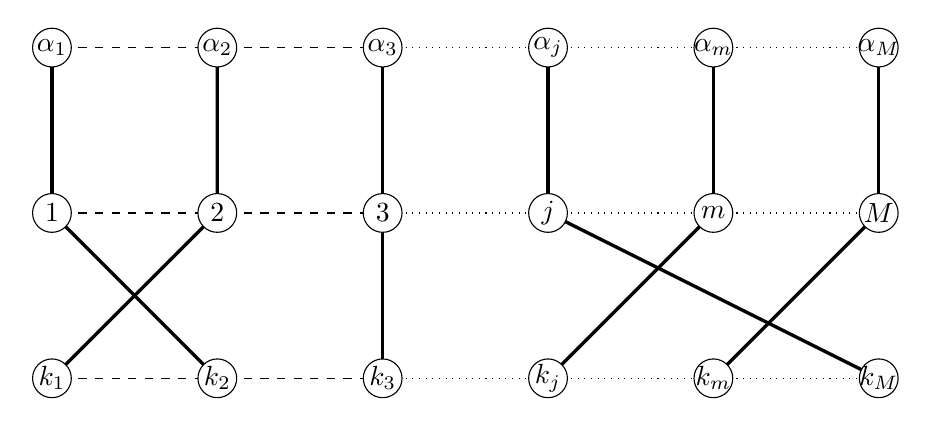
\begin{tikzpicture}[scale=0.7]


\node (alfa1) at (-10,6) {};
\node (alfaM) at (5,6) {};
\node (alfa2)at (-7,6) {};
\node (alfa3) at (-4,6) {};
\node (alfa4)at (-1,6) {};
\node (alfa5)at (2,6) {};

\node (v1) at (-10,3) {};
\node (vM) at (5,3) {};
\node (v2)at (-7,3) {};
\node (v3) at (-4,3) {};
\node (v4)at (-1,3) {};
\node (v5)at (2,3) {};

\node (k1) at (-10,0) {};
\node (kM) at (5,0) {};
\node (k2)at (-7,0) {};
\node (k3) at (-4,0) {};
\node (k4)at (-1,0) {};
\node (k5)at (2,0) {};


\draw[very thick]  (alfa1) --(v1);
\draw[very thick]  (alfa2) --(v2);
\draw[very thick]  (alfa3) --(v3);
\draw[very thick]  (alfa4) --(v4);
\draw[very thick]  (alfa5) --(v5);
\draw[very thick]  (alfaM) --(vM);
\draw[very thick]  (k2) --(v1);
\draw[very thick]  (k1) --(v2);
\draw[very thick]  (k3) --(v3);
\draw[very thick]  (kM) --(v4);
\draw[very thick]  (k4) --(v5);
\draw[very thick]  (k5) --(vM);



\draw[dashed]  (alfa1) --(alfa2);
\draw[dashed]  (alfa2) --(alfa3);
\draw[dotted]  (alfa3) --(alfa4);
\draw[dotted]  (alfa4) --(alfa5);
\draw [dotted](alfa5) --(alfaM);

\draw  [fill= white](alfa1)circle (10pt);
\draw  [fill= white](alfaM)circle (10pt);
\draw  [fill= white](alfa2)circle (10pt);
\draw  [fill= white](alfa3)circle (10pt);
\draw  [fill= white](alfa4)circle (10pt);
\draw  [fill= white](alfa5)circle (10pt);

\node[] at (alfa1)  {$\alpha_1$};
\node[] at (alfaM)  {$\alpha_M$};
\node[] at (alfa2)  {$\alpha_2$};
\node[] at (alfa3)  {$\alpha_3$};
\node[] at (alfa4)  {$\alpha_j$};
\node[] at (alfa5)  {$\alpha_m$};



\draw [dashed] (v1) --(v2);
\draw[dashed]  (v2) --(v3);
\draw[dotted]  (v3) --(v4);
\draw[dotted]  (v4) --(v5);

\draw  [dotted](v5) --(vM);
\draw  [fill= white](v1)circle (10pt);
\draw  [fill= white](vM)circle (10pt);
\draw  [fill= white](v2)circle (10pt);
\draw  [fill= white](v3)circle (10pt);
\draw  [fill= white](v4)circle (10pt);
\draw  [fill= white](v5)circle (10pt);

\node[] at (v1)  {$1$};
\node[] at (vM)  {$M$};
\node[] at (v2)  {$2$};
\node[] at (v3)  {$3$};
\node[] at (v4)  {$j$};
\node[] at (v5)  {$m$};



\draw[dashed]  (k1) --(k2);
\draw[dashed]  (k2) --(k3);
\draw[dotted]  (k3) --(k4);
\draw[dotted]  (k4) --(k5);

\draw  [dotted](k5) --(kM);
\draw  [fill= white](k1)circle (10pt);
\draw  [fill= white](kM)circle (10pt);
\draw  [fill= white](k2)circle (10pt);
\draw  [fill= white](k3)circle (10pt);
\draw  [fill= white](k4)circle (10pt);
\draw  [fill= white](k5)circle (10pt);

\node[] at (k1)  {$k_1$};
\node[] at (kM)  {$k_M$};
\node[] at (k2)  {$k_2$};
\node[] at (k3)  {$k_3$};
\node[] at (k4)  {$k_j$};
\node[] at (k5)  {$k_m$};


\end{tikzpicture}}\\
    \subfloat[]{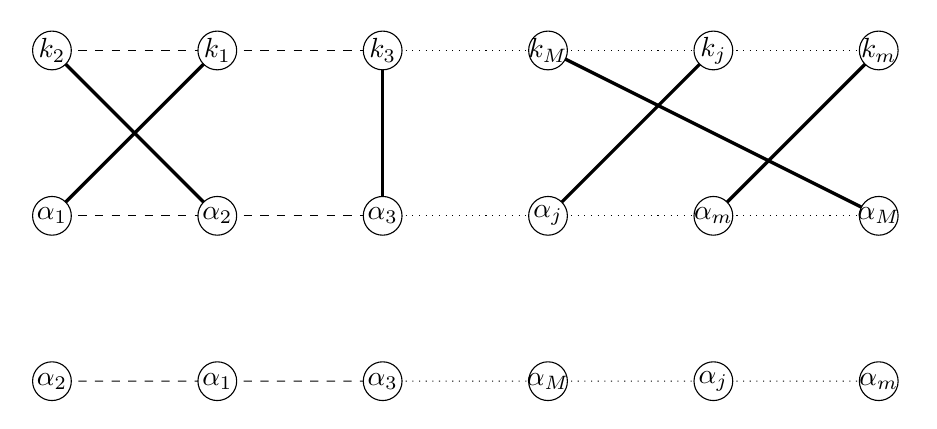
\begin{tikzpicture}[scale=0.7]


\node (alfaPR1) at (-10,-9) {};
\node (alfaPRM) at (5,-9) {};
\node (alfaPR2)at (-7,-9) {};
\node (alfaPR3) at (-4,-9) {};
\node (alfaPR4)at (-1,-9) {};
\node (alfaPR5)at (2,-9) {};

\node (alfaP1) at (-10,-6) {};
\node (alfaPM) at (5,-6) {};
\node (alfaP2)at (-7,-6) {};
\node (alfaP3) at (-4,-6) {};
\node (alfaP4)at (-1,-6) {};
\node (alfaP5)at (2,-6) {};

\node (kp1) at (-10,-3) {};
\node (kpM) at (5,-3) {};
\node (kp2)at (-7,-3) {};
\node (kp3) at (-4,-3) {};
\node (kp4)at (-1,-3) {};
\node (kp5)at (2,-3) {};



\draw[very thick]  (alfaP2) --(kp1);
\draw[very thick]  (alfaP1) --(kp2);
\draw[very thick]  (alfaP3) --(kp3);
\draw[very thick]  (alfaPM) --(kp4);
\draw[very thick]  (alfaP4) --(kp5);
\draw[very thick]  (alfaP5) --(kpM);



\draw [dashed] (kp1) --(kp2);
\draw [dashed] (kp2) --(kp3);
\draw[dotted]  (kp3) --(kp4);
\draw[dotted]  (kp4) --(kp5);
\draw  [dotted](kp5) --(kpM);

\draw  [fill= white](kp1)circle (10pt);
\draw  [fill= white](kpM)circle (10pt);
\draw  [fill= white](kp2)circle (10pt);
\draw  [fill= white](kp3)circle (10pt);
\draw  [fill= white](kp4)circle (10pt);
\draw  [fill= white](kp5)circle (10pt);

\node[] at (kp1)  {$k_2$};
\node[] at (kpM)  {$k_m$};
\node[] at (kp2)  {$k_1$};
\node[] at (kp3)  {$k_3$};
\node[] at (kp4)  {$k_M$};
\node[] at (kp5)  {$k_j$};

\draw[dashed]  (alfaP1) --(alfaP2);
\draw[dashed]  (alfaP2) --(alfaP3);
\draw[dotted]  (alfaP3) --(alfaP4);
\draw[dotted]  (alfaP4) --(alfaP5);
\draw [dotted](alfaP5) --(alfaPM);

\draw[dashed]  (alfaPR1) --(alfaPR2);
\draw[dashed]  (alfaPR2) --(alfaPR3);
\draw[dotted]  (alfaPR3) --(alfaPR4);
\draw[dotted]  (alfaPR4) --(alfaPR5);
\draw [dotted](alfaPR5) --(alfaPRM);

\draw  [fill= white](alfaP1)circle (10pt);
\draw  [fill= white](alfaPM)circle (10pt);
\draw  [fill= white](alfaP2)circle (10pt);
\draw  [fill= white](alfaP3)circle (10pt);
\draw  [fill= white](alfaP4)circle (10pt);
\draw  [fill= white](alfaP5)circle (10pt);

\draw  [fill= white](alfaPR1)circle (10pt);
\draw  [fill= white](alfaPRM)circle (10pt);
\draw  [fill= white](alfaPR2)circle (10pt);
\draw  [fill= white](alfaPR3)circle (10pt);
\draw  [fill= white](alfaPR4)circle (10pt);
\draw  [fill= white](alfaPR5)circle (10pt);

\node[] at (alfaP1)  {$\alpha_1$};
\node[] at (alfaPM)  {$\alpha_M$};
\node[] at (alfaP2)  {$\alpha_2$};
\node[] at (alfaP3)  {$\alpha_3$};
\node[] at (alfaP4)  {$\alpha_j$};
\node[] at (alfaP5)  {$\alpha_m$};

\node[] at (alfaPR1)  {$\alpha_2$};
\node[] at (alfaPRM)  {$\alpha_m$};
\node[] at (alfaPR2)  {$\alpha_1$};
\node[] at (alfaPR3)  {$\alpha_3$};
\node[] at (alfaPR4)  {$\alpha_M$};
\node[] at (alfaPR5)  {$\alpha_j$};
\end{tikzpicture}}
\caption{Permutations}
\label{fig:fig_p255}
\end{figure}
Indeed suppose, as in the example $(a)$ ,  $k_1=2, k_2=1,k_3=3, ,\dots ,k_j = m,\dots , k_m=j,\dots$ etc., so we get a sequence $\{k_2, k_1,k_3,\dots, k_m,\dots k_j,\dots\}$ as illustrate in $(b)$. But to have - with this sequence - an equivalent expression of 
$d\tau_{(M)}^{k_1 k_2\dots k_m}=(\theta_{\alpha}) \delta_{1 2 \dots M}^{\alpha_1\dots \alpha_M}d_{(\alpha_1)}x^{k_j}d_{(\alpha_2)}x^{k_m}\dots d_{(\alpha_M)}x^{k_n}$, we need to make an equivalent permutation so that $\alpha_r$ gets in the same position  as $k_r$, resulting in a new sequence $\{\alpha_2,\alpha_1,\alpha_3,\dots,\alpha_M,\dots,\alpha_j, \alpha_m\}$.\\
The number of permutations to generate $\theta_{\alpha}$ and $\theta_k$ are identical resulting in $\theta_{\alpha}\theta_k=1$.
So $(6)$ can be rewritten (noting that the $\alpha_r$ are dummy indexes and that we are free to rename them so that $r=1, n=2,\dots$) 
\begin{align}
d\tau_{(M)}^{k_1 k_2\dots k_m}= \delta_{1 2 \dots M}^{\beta_1\beta_2 \dots \beta_M}d_{(\beta_1)}x^{k_1}d_{(\beta_2)}x^{k_2}\dots d_{(\beta_n)}x^{k_n}\dots d_{(\beta_M)}x^{k_M}
\end{align}
Finally, using $\mathbf{7.114}$ 
\begin{align}
d\tau_{(M)}^{k_1 k_2\dots k_m}&= \underbrace{\epsilon_{1 2 \dots M}}_{=1}\epsilon^{\beta_1\beta_2 \dots \beta_M}d_{(\beta_1)}x^{k_1}d_{(\beta_2)}x^{k_2}\dots d_{(\beta_n)}x^{k_n}\dots d_{(\beta_M)}x^{k_M}\\
&= \epsilon^{\beta_1\beta_2 \dots \beta_M}d_{(\beta_1)}x^{k_1}d_{(\beta_2)}x^{k_2}\dots d_{(\beta_n)}x^{k_n}\dots d_{(\beta_M)}x^{k_M}
\end{align}
$$\blacklozenge$$
\newpage

